\documentclass{article}
\usepackage{epsfig, latexsym}


\begin{document}

\newcommand{\SOPmin}{${\rm SOP}_{\rm min} \ $}
\newcommand{\POSmin}{${\rm POS}_{\rm min} \ $}
\newcommand{\bs}{\backslash}


\title{
\Huge{CSE 271 -- Fall 2004}\\
\normalsize{Exam 2}\\
\makebox[4in][l]{Name:} SSN:}
\date{}

\maketitle{}

\begin{tabular}{llll}
\begin{tabular}{c||c}
D & Q+   \\ \hline
0 & 0 \\ \hline
1 & 1 \\
\end{tabular}
&
\begin{tabular}{c||c}
T & Q+   \\ \hline
0 & Q \\ \hline
1 & Q' \\
\end{tabular}
&
\begin{tabular}{c|c||c}
S & R & Q+   \\ \hline
0 & 0 & Q \\ \hline
0 & 1 & 0 \\ \hline
1 & 0 & 1 \\ \hline
1 & 1 & x \\
\end{tabular}
&
\begin{tabular}{c|c||c}
J & K & Q+   \\ \hline
0 & 0 & Q \\ \hline
0 & 1 & 0 \\ \hline
1 & 0 & 1 \\ \hline
1 & 1 & Q' \\
\end{tabular}
\\
\end{tabular}

\begin{tabular}{ll}
All counter in this exam are  &
All shift registers in this \\

4-bits wide and have the  &
exam are 4-bits wide and \\

following behavior. &
have the following behavior.  \\ 

\begin{tabular}{l|l|l||l}
clk             & $C_1 C_0$     & D & $Q^+$     \\ \hline
0,1,$\downarrow$& xx            & x & Q         \\ \hline
$\uparrow$      & 00            & x & Q         \\  \hline
$\uparrow$      & 01            & x & Q+1	\\  \hline
$\uparrow$      & 10            & x & Q-1	\\  \hline
$\uparrow$      & 11            & D & D         \\
\end{tabular}
& 
\begin{tabular}{l|l|l||l|r}
clk         & $C_1 C_0$ & D & $Q^+$ & comment \\ \hline \hline
0,1,$\downarrow$ & xx   & x & Q     & hold     \\ \hline
$\uparrow$     & 00     & x & Q     & hold     \\  \hline
$\uparrow$     & 01     & x & Q$>>$1 & shift right \\  \hline
$\uparrow$     & 10     & x & Q$<<$1 & shift left \\  \hline
$\uparrow$     & 11     & D & D     & parallel load  \\
\end{tabular} \\ 
\end{tabular} 


\begin{enumerate}

\item {\bf (1 pt.)} Assuming a word size of 5 bits, interpret 10101 as a 2's complement
number.

\begin{tabular}{p{0.6in} p{0.6in} p{0.6in} p{0.6in} l}
a) -21 & b) -11 & c) -10 & d) -5 & e) None of the above
\end{tabular}

\item {\bf (1 pt.)} Assuming a word size of 5 bits, determine the 2's complement
representation of -12.

\begin{tabular}{p{0.6in} p{0.6in} p{0.6in} p{0.6in} l}
a) 10100 & b) 11100 & c) 10011 & d) 10010 & e) None of the above
\end{tabular}

\item {\bf (1 pt.)}How many OR gates are there inside a 3:8 decoder?

\begin{tabular}{p{0.6in} p{0.6in} p{0.6in} p{0.6in} l}
a) 1 & b) 3 & c) 8 & d) 16 & e) None of the above
\end{tabular}

\item {\bf (1 pt.)}How many inputs do the AND gates inside a 3:8 decoder have?

\begin{tabular}{p{0.6in} p{0.6in} p{0.6in} p{0.6in} l}
a) 1 & b) 3 & c) 4 & d) 8 & e) None of the above
\end{tabular}

\item {\bf (1 pt.)} How many AND gates are there in an 8:1 mux?

\begin{tabular}{p{0.6in} p{0.6in} p{0.6in} p{0.6in} l}
a) 1 & b) 2 & c) 3 & d) 8 & e) None of the above
\end{tabular}

\pagebreak
\item {\bf (1 pt.)} How many 2:1 muxes are needed to construct a 64x1 mux?

\begin{tabular}{p{0.6in} p{0.6in} p{0.6in} p{0.6in} l}
a) 31 & b) 32 & c) 63 & d) 64 & e) None of the above
\end{tabular}

\vspace{0.1in}

You are given the following 4:16 decoder built from 2:4 decoders.  
Unfortunately, the student who built it wired the select lines in a 
most unusual fashion.  Its your job to label each output with the 
index which selects it.  Most of the outputs have been omitted 
for clarity.

\scalebox{0.7}{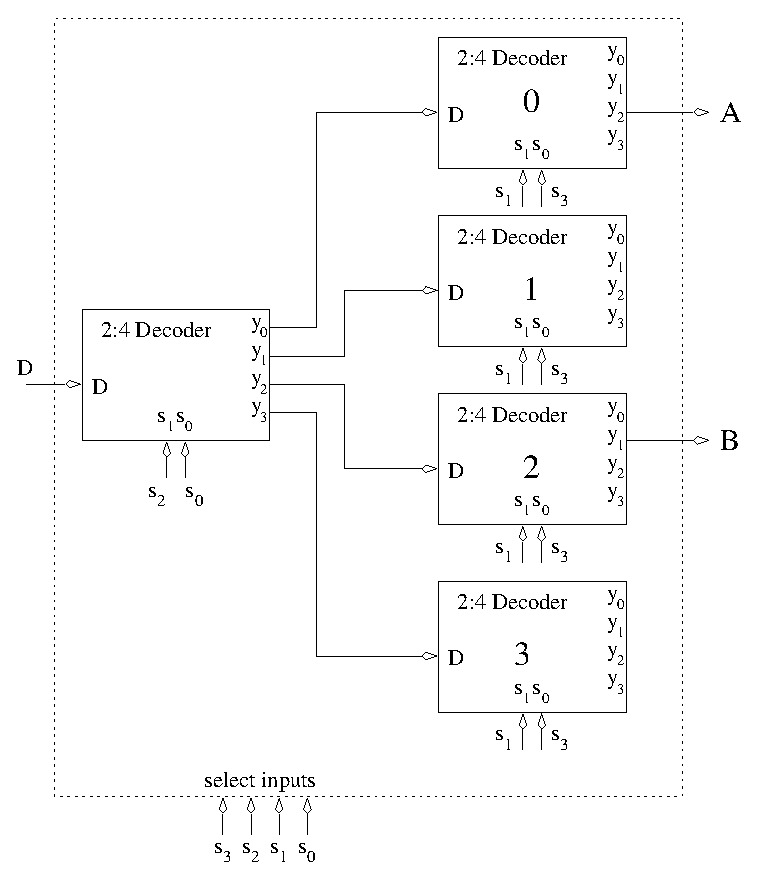
\includegraphics{./Fig2/OddDecoder}}

\item {\bf (1 pt.)} What is the value of the output labeled A?

\begin{tabular}{p{0.6in} p{0.6in} p{0.6in} p{0.6in} l}
a) $y_{1}$ & b) $y_{2}$ & c) $y_{4}$ & d) $y_{8}$ & e) None of the above
\end{tabular}

\item {\bf (1 pt.)} What is the value of the output labeled B?

\begin{tabular}{p{0.6in} p{0.6in} p{0.6in} p{0.6in} l}
a) $y_{1}$ & b) $y_{6}$ & c) $y_{9}$ & d) $y_{12}$ & e) None of the above
\end{tabular}

\pagebreak
\item {\bf (2 pt.)} Which line of pseudo-code best characterizes
the following piece of hardware.

\scalebox{0.7}{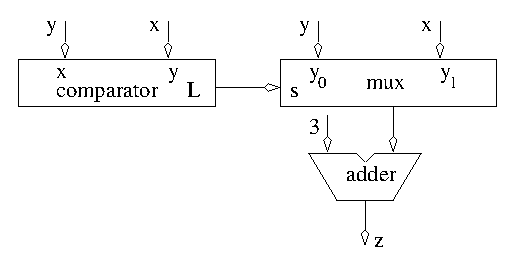
\includegraphics{./Fig2/conditional}}

\begin{description}
\item{a) } \verb^if (X < Y) then Z = X+3 else Z = Y+3;^
\item{b) } \verb^if (X < Y) then Z = Y+3 else Z = X+3;^
\item{c) } \verb^if (X > Y) then Z = X+3 else Z = Y+3;^
\item{d) } \verb^if (X > Y) then Z = Y+3 else Z = X+3;^
\item{e) } None of the above
\end{description}


For questions 10-11 you are to complete the state table 
for the following circuit.

\scalebox{0.7}{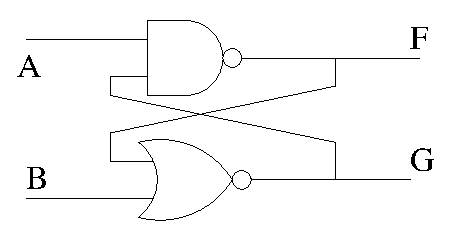
\includegraphics{./Fig2/cross}}

\item {\bf (1 pt.)} What does $G^+$ equal for (A,B)=(0,0)?

\begin{tabular}{p{0.6in} p{0.6in} p{0.6in} p{0.6in} l}
a) 0 & b) 1 & c) F & d) F' & e) illegal
\end{tabular}

\item {\bf (1 pt.)} What does $F^+$ equal for (A,B)=(1,1)?

\begin{tabular}{p{0.6in} p{0.6in} p{0.6in} p{0.6in} l}
a) 0 & b) 1 & c) F & d) F' & e) illegal
\end{tabular}

\item {\bf (2 pt.)}What is the logic inside \verb+ box + in order
to make the count sequence on Q go from 3 to 10 (inclusive of both)
over and over.

\includegraphics[-60mm,23mm][0mm,30.1mm]{./Fig2/OddCnt}

\begin{description}
\item{a) }$c_1 = L' \hspace{0.2in} c_0=0$ 
\item{b) }$c_1 = L' \hspace{0.2in} c_0=1$ 
\item{c) }$c_1 = L  \hspace{0.2in} c_0=0$ 
\item{d) }$c_1 = L  \hspace{0.2in} c_0=1$ 
\item{e) }None of the above
\end{description}

\pagebreak
For questions 13-16 use the circuit and timing diagram
show below.  If necessary, you can assume that Q settles to 0 
after a period of rapid toggling.

\scalebox{0.7}{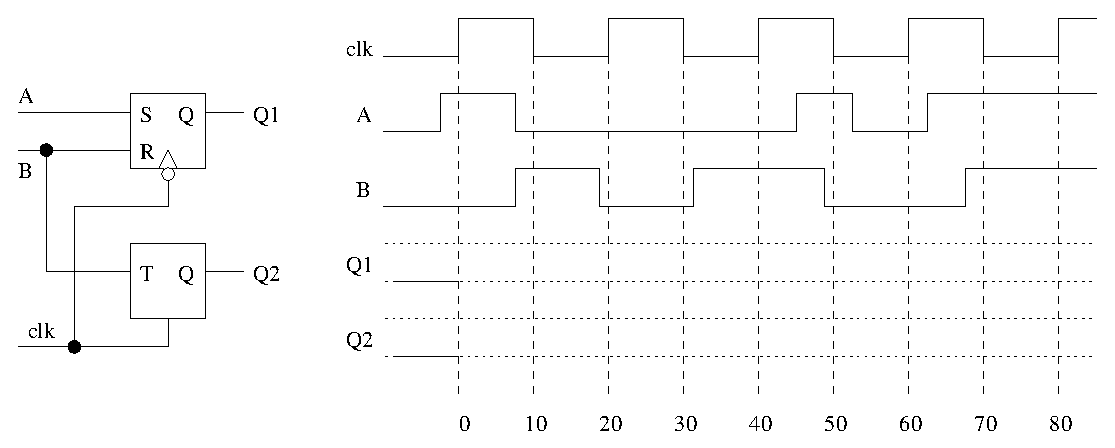
\includegraphics{./Fig2/ExTim4}}

\item {\bf (1 pt.)} What is the value of $Q_1$ at time=25nS?

\begin{tabular}{p{0.6in} p{0.6in} p{1.2in} l}
a) 0 & b) 1 & c) Toggling rapidly & d) Unknown 
\end{tabular}

\item {\bf (1 pt.)} What is the value of $Q_1$ at time=75nS?

\begin{tabular}{p{0.6in} p{0.6in} p{1.2in} l}
a) 0 & b) 1 & c) Toggling rapidly & d) Unknown 
\end{tabular}

\item {\bf (1 pt.)} What is the value of $Q_2$ at time=15nS?

\begin{tabular}{p{0.6in} p{0.6in} p{1.2in} l}
a) 0 & b) 1 & c) Toggling rapidly & d) Unknown 
\end{tabular}

\item {\bf (1 pt.)} What is the value of $Q_2$ at time=45nS?

\begin{tabular}{p{0.6in} p{0.6in} p{1.2in} l}
a) 0 & b) 1 & c) Toggling rapidly & d) Unknown 
\end{tabular}


\pagebreak
For problems 17-19 use the timing diagram below as the 
input to a counter.  Determine the output sequence Q to answer 
the questions below.

\scalebox{0.7}{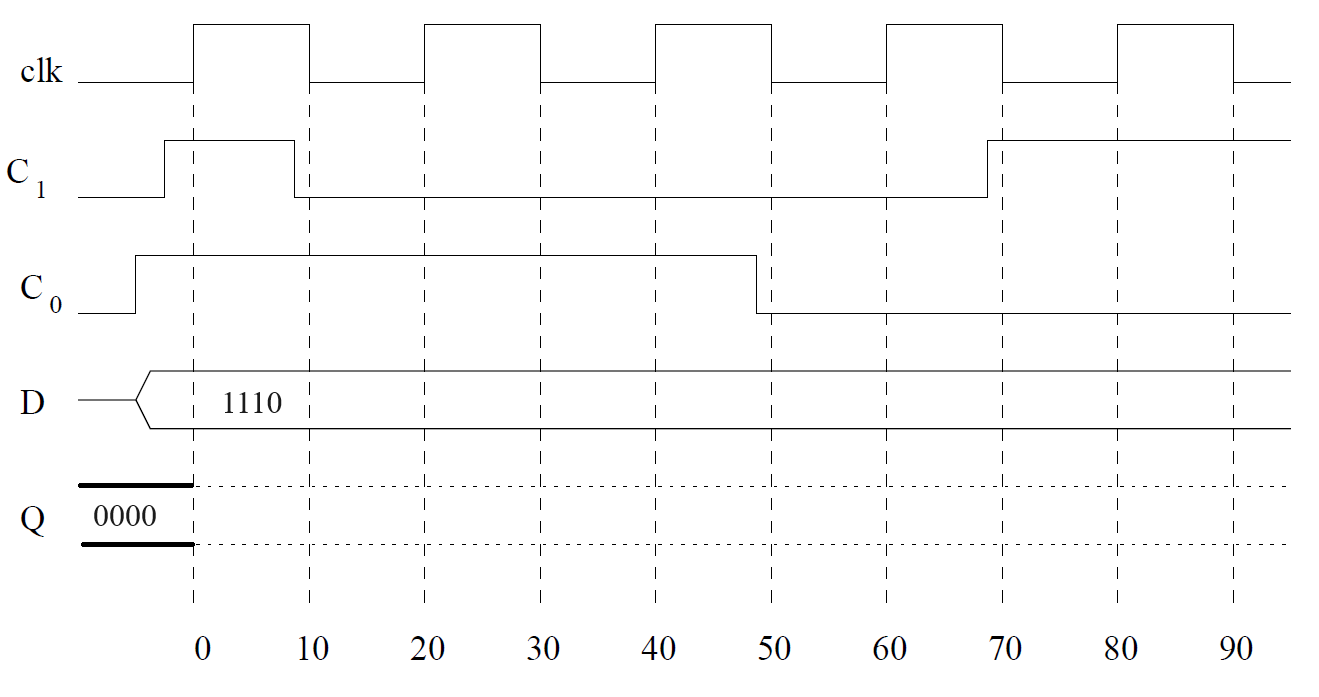
\includegraphics{./Fig2/CntTime}}

\item {\bf (1 pt.)}What is the value of $Q$ at time 15?

\begin{tabular}{p{0.6in} p{0.6in} p{0.6in} p{0.6in} l}
a) 0000 & b) 0001 & c) 1110 & d) 1111 & e) None of the above
\end{tabular}

\item {\bf (1 pt.)}What is the value of $Q$ at time 65?

\begin{tabular}{p{0.6in} p{0.6in} p{0.6in} p{0.6in} l}
a) 0000 & b) 0001 & c) 1110 & d) 1111 & e) None of the above
\end{tabular}

\item {\bf (1 pt.)}What is the value of $Q$ at time 85?

\begin{tabular}{p{0.6in} p{0.6in} p{0.6in} p{0.6in} l}
a) 0000 & b) 0001 & c) 1110 & d) 1111 & e) None of the above
\end{tabular}

For problems 20-22 use the timing diagram below as the input to a arithmetic 
shift register.  Determine the output sequence Q to answer the questions
below.

\scalebox{0.7}{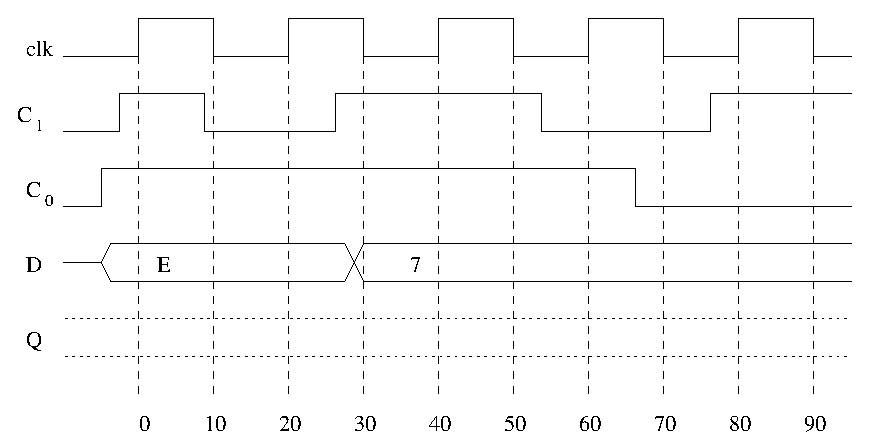
\includegraphics{./Fig2/SftTime}}

\item {\bf (1 pt.)}What is the value of $Q$ at time 25?

\begin{tabular}{p{0.6in} p{0.6in} p{0.6in} p{0.6in} l}
a) 0000 & b) 0111 & c) 1110 & d) 1111 & e) None of the above
\end{tabular}

\item {\bf (1 pt.)}What is the value of $Q$ at time 65?

\begin{tabular}{p{0.6in} p{0.6in} p{0.6in} p{0.6in} l}
a) 0000 & b) 0111 & c) 0110 & d) 1110 & e) None of the above
\end{tabular}

\item {\bf (1 pt.)}What is the value of $Q$ at time 85?

\begin{tabular}{p{0.6in} p{0.6in} p{0.6in} p{0.6in} l}
a) 0000 & b) 0111 & c) 0110 & d) 1110 & e) None of the above
\end{tabular}

\pagebreak
For problems 23-27 use the following figure and timing diagram.
You should assume that all the devices process 5-bits data 
values.

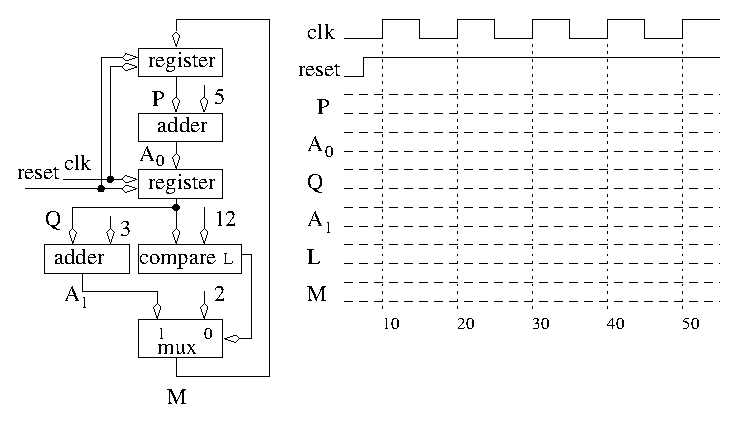
\includegraphics{./Fig2/BBBtiming2}

\item {\bf (2 pt.)}What is the value of $P$ at time 15?

\begin{tabular}{p{0.6in} p{0.6in} p{0.6in} p{0.6in} l}
a) 0 & b) 2 & c) 3 & d) 5 & e) 8
\end{tabular}

\item {\bf (2 pt.)}What is the value of $A_0$ at time 25?

\begin{tabular}{p{0.6in} p{0.6in} p{0.6in} p{0.6in} l}
a) 7 & b) 8 & c) 11 & d) 13 & e) 16
\end{tabular}

\item {\bf (2 pt.)}What is the value of $Q$ at time 35?

\begin{tabular}{p{0.6in} p{0.6in} p{0.6in} p{0.6in} l}
a) 7 & b) 8 & c) 11 & d) 13 & e) 16
\end{tabular}

\item {\bf (2 pt.)}What is the value of $A_1$ at time 45?

\begin{tabular}{p{0.6in} p{0.6in} p{0.6in} p{0.6in} l}
a) 8 & b) 10 & c) 13 & d) 16 & e) 19
\end{tabular}

\item {\bf (2 pt.)}What is the value of $M$ at time 55?

\begin{tabular}{p{0.6in} p{0.6in} p{0.6in} p{0.6in} l}
a) 2 & b) 8 & c) 10 & d) 11 & e) 12
\end{tabular}

\end{enumerate}
\end{document}
